\section{Design of the Protocol}
\label{sec:secure-design}

Since the attacks described in the previous section (allowing a malicious retailer to exploit a customer)
	are tied to the retailer's ability to display one price and charge another,
	our proposed defense against these attacks is built around removing this ability.
If using a credit card implemented on a smart phone, the phone's interface provides an additional communication channel between the customer and the credit card.
In this case we refer to the card as a ``virtual'' credit card.
The communication channel between the smart phone and the customer can be harnessed to allow the customer to participate in the credit card protocol,
	beyond simply allowing it to occur.

The Externally Secure CC Protocol described in Chapter \ref{cha:external} defines a function \emph{H},
    proves several of its properties, and uses it to defend against external attacks such as skimming and eavesdropping.
We note that each property required of this function \emph{H} is a property enjoyed by common cryptographic hash functions,
    such as those in the \emph{SHA} family.
As such, using a hash function instead of the derived function \emph{H} does not reduce the security of the Secure CC Protocol.
In the context of virtual credit cards, the computational cost of executing a hash function is no longer a concern.

We remind the reader of the following terms:

\begin{description}
\item[ch:] a fresh, randomly generated challenge value, chosen by the point of sale.
\item[info:] the credit card's payment information, consisting of the credit card number and expiration date.
\item[ID:] a UUID, uniquely identifying an individual credit card without revealing any information about \emph{info}.
	This identifier is stored as a constant on the credit card.
\item[iCVV:] an unpredictable value freshly generated by the credit card for each transaction (the issuing bank can generate the same sequence of values).
\item[B:] the name of the issuing bank, used for the purpose of routing transactions as before.
\item[T:] a charge token, to authenticate a single transaction.
\end{description}

The Secure CC Protocol, operating between a point of sale and a virtual credit card, is illustrated in Figure \ref{fig:secure-ccp} and proceeds as follows:

\begin{enumerate}
\item The point of sale displays a price \val{\$d} on its screen, inviting the customer to bring his credit card within NFC range.
\item The point of sale sends a Solicitation message to the credit card, including a fresh random challenge \val{ch} and the price to be charged \val{\$s}.
	(Recall that if the point of sale is honest, \val{\$s} = \val{\$d})
\item The virtual credit card displays the price \val{\$s} on the smart phone to the customer, who can choose to accept or reject it.
	Rejecting the price aborts the protocol here.
\item If the price is accepted by the customer, the virtual credit card calculates
    $$T = H(\textrm{\emph{info}},~ ch,~ \textrm{\emph{\$s}},~ \textrm{\emph{iCVV}})$$
	and responds to the point of sale with a Card Information message consisting of (\val{ID}, \val{T}, \val{B}).
\item The point of sale sends a charge request message to the issuing bank (identified by \val{B}) consisting of (\val{ID}, \val{T}, \val{ch}, \val{\$r}).
	(Again, if the point of sale is honest, \val{\$r} = \val{\$d})
\item The bank uses \val{ID} to look up \emph{info\textsubscript{bank}} and then calculates \emph{iCVV\textsubscript{bank}}.
	It then uses the \val{ch} and \val{\$r} supplied in the charge request message to determine
	$$T_{bank} = H(\textrm{\emph{info}}_{bank},~ ch,~ \textrm{\emph{\$r}},~ \textrm{\emph{iCVV}}_{bank})$$
	If $T \neq T_{\text{bank}}$, the bank will decline the charge, otherwise it approves the charge for \val{\$r}.
\end{enumerate}

\begin{figure}
  \caption{Secure CC Protocol}
  \centering
    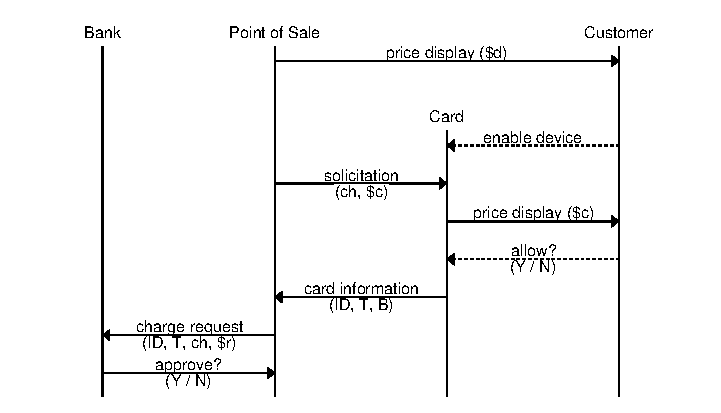
\includegraphics{img/secure_ccp.eps}
  \label{fig:secure-ccp}
\end{figure}

When using a physical credit card instead of a virtual one, no communication channel exists between the card and the customer.
As a result, the steps above in which the card displays the price sent with the Solicitation message (\val{\$s}) to the customer and waits for the customer to allow the protocol to proceed cannot occur.
Instead, a physical credit card must implicitly assume successful authorization from the customer, effectively skipping step 3.
As a result, while not providing protections from malicious retailers to physical credit cards, the protocol maintains backwards compatibility with no loss of functionality or security against malicious outsiders.

We note that a naive implementation of the protocol above might require excessively long timeouts between the point of sale sending its solicitation message and receiving the response.
Should long timeouts not be desired, a simple solution would be for the point of sale to send periodic solicitations (with new challenges).
The virtual credit card, upon receiving permission from the customer, could then cache this approval and respond immediately to the subsequent solicitation.
Besides noting this particular case, we emphasize that issues such as these are implementation details, the decisions for which are best left to those implementing the protocol.

\subsection{Defending Against the Over-charge Attack}

The Secure CC Protocol prevents the Over-charge attack against customers using a virtual credit card.
In step 3, the customer verifies that \linebreak \val{\$d} = \val{\$s} through visual comparison.
Due to the inclusion of \val{\$s} in the hash when generating token \emph{T}, we gain the assurance that for any charge accepted by the bank, \val{\$s} = \val{\$r}.

Thus, through a transitive argument, the customer can be assured that for any successful charge, \val{\$d} = \val{\$r}.
Should the malicious retailer attempt to issue a charge request with some $\textrm{\emph{\$r}} \neq \textrm{\emph{\$d}}$, then $T_{bank} \neq T$ and the charge will be declined by the bank.

\subsection{Defending Against the Transparent Bridge Attack}

The Secure CC Protocol makes no attempt to prevent this attack from occurring.
Instead, it removes the economic incentive of performing such an attack against customers using virtual credit cards.

In the Transparent Bridge attack, the malicious retailer loses the sale paid by the victim customer, in return for acquiring the purchase made by the malicious customer.
In order for the Transparent Bridge attack to be viable, the malicious actors must have something to gain:
  the value of the malicious customer's purchase must be greater than the value of the victim customer's purchase.
When the Secure CC Protocol is used, one of two scenarios occurs:

\begin{enumerate}
\item The price associated with the malicious customer's purchase differs from (i.e. is greater than) the price of the victim customer's purchase.
The victim customer compares the price displayed by the point of sale and the price displayed by his virtual credit card.
The would-be victim customer immediately detects the attack and aborts the transaction.
\item The price associated with the malicious customer's purchase is equal to the price of the victim customer's purchase.
The victim customer does not detect this attack, and allows the transaction to occur.
The end result: the victim customer paid for the price of what he received, and the victim retailer received the price of what it sold.
\end{enumerate}

As a result, there is no longer any incentive to carrying out this attack, as the only successful instance results in all parties getting paid exactly as much as they would had they been honest.
